\documentclass[
  25pt,
  a0paper,
  landscape,
  margin=18mm,
  innermargin=15mm,
  blockverticalspace=15mm,
  colspace=15mm
]{tikzposter}

\usepackage[utf8]{inputenc}
\usepackage{graphicx}
\usepackage{amsmath,amssymb}
\usepackage{booktabs}
\usepackage{microtype}

% Theme and Color Style
\usetheme{Default}
\usecolorstyle{Denmark}

% Custom Colors (USTH Navy & Academic Gold)
\definecolorstyle{USTHStyle}{
  \definecolor{navyBlue}{RGB}{10, 37, 64}
  \definecolor{accentGold}{RGB}{217, 119, 6}
  \definecolor{lightBg}{RGB}{248, 250, 252}
  \definecolor{darkSlate}{RGB}{30, 41, 59}
}{
  % Background Colors
  \colorlet{backgroundcolor}{lightBg}
  \colorlet{framecolor}{navyBlue}
  % Title Colors
  \colorlet{titlefgcolor}{white}
  \colorlet{titlebgcolor}{navyBlue}
  % Block Colors
  \colorlet{blocktitlebgcolor}{navyBlue}
  \colorlet{blocktitlefgcolor}{white}
  \colorlet{blockbodybgcolor}{white}
  \colorlet{blockbodyfgcolor}{darkSlate}
}
\usecolorstyle{USTHStyle}

% Title, Authors, and Institute
\title{\textbf{Design and Fabrication of Low-Temperature Continuous-Flow Cryostat System}}
\author{Nguyen Xuan Tai, Nguyen Tien Dat, Tran Phan Sang, Nguyen Minh Tam}
\institute{
  Department of Advanced Materials Science and Nanotechnology, University of Science and Technology of Hanoi (USTH) \\
  \textit{Instructors: Dr. Nguyen Van Quyen (AMSN, USTH) $\cdot$ Nguyen Van Huan (An Tai Loc Co., Ltd.)}
}
\titlegraphic{
\includegraphics[height=5.2cm]{usth_logo.png}}

\begin{document}

\maketitle[width=0.98\textwidth]

\begin{columns}

  % ============================================================================
  % COLUMN 1: MOTIVATION & THERMODYNAMICS
  % ============================================================================
  \column{0.33}

  \block{1. Motivation \& Physical Principles}{
    Cryogenic environments ($77\text{ K} - 300\text{ K}$) are indispensable for investigating low-dimensional quantum transport, semiconductor devices, and phase transitions. Conventional commercial cryostats are cost-prohibitive for flexible laboratory prototyping.

    \vspace{0.4cm}
    \textbf{Core Objective:} Develop a customizable, modular continuous-flow cryostat operating between $77\text{ K}$ and $300\text{ K}$ with high-vacuum isolation ($P < 10^{-4}\text{ mbar}$) and in-situ 4-probe electrical transport tracking.

    \vspace{0.6cm}
    \textbf{Thermodynamic Heat Balance:}
    \begin{equation*}
      \dot{Q}_{\text{total}} = \dot{Q}_{\text{cond}} + \dot{Q}_{\text{rad}} + \dot{Q}_{\text{conv}}
    \end{equation*}
    \begin{itemize}
      \item \textbf{Conduction Leakage:} Fourier's Law with temperature-dependent $k(T)$:
      \begin{equation*}
        \dot{Q}_{\text{cond}} = \frac{A}{L} \int_{T_C}^{T_H} k(T)\,dT
      \end{equation*}
      \item \textbf{Radiation Transfer:} Stefan-Boltzmann law with radiation baffles:
      \begin{equation*}
        \dot{Q}_{\text{rad}} = \epsilon \sigma A (T_H^4 - T_C^4)
      \end{equation*}
      \item \textbf{High Vacuum Molecular Flow:} At $P \le 10^{-4}\text{ mbar}$, molecular mean free path exceeds chamber dimensions $\implies \dot{Q}_{\text{conv}} \approx 0$.
    \end{itemize}
  }

  \block{2. Materials \& Thermal Coupling}{
    \begin{center}
      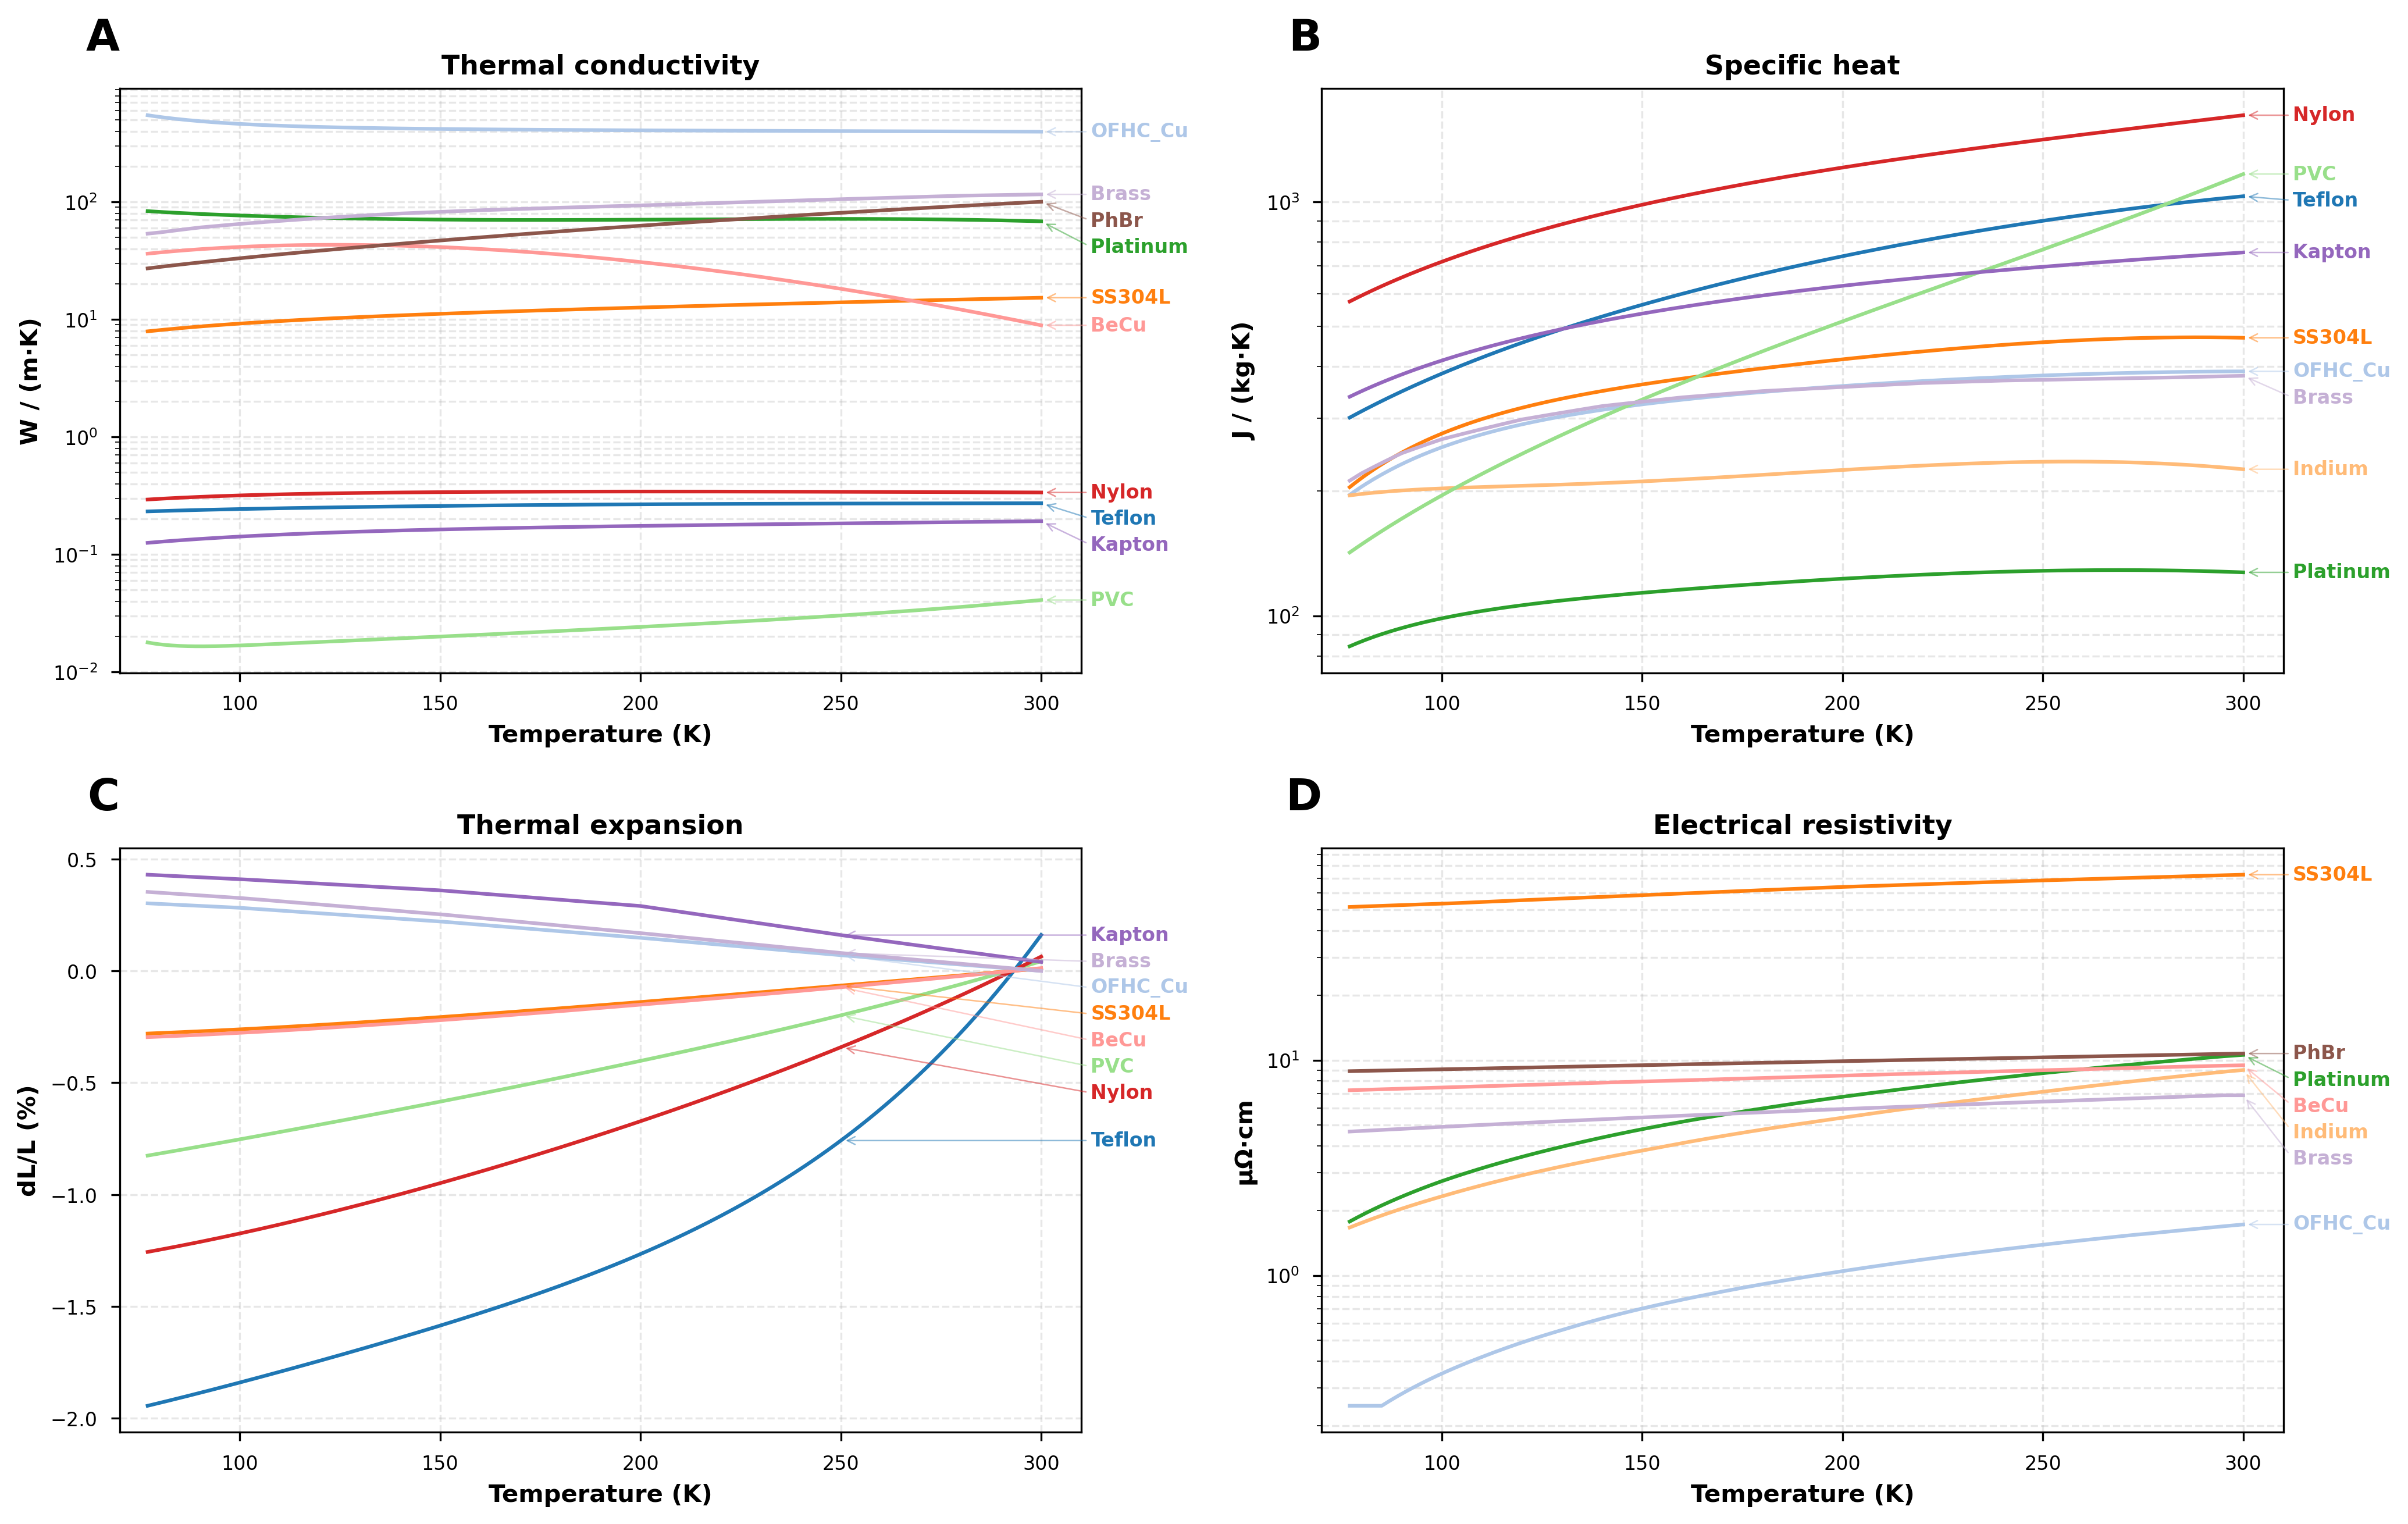
\includegraphics[width=0.92\linewidth]{cryostat_materials_properties.png} \\
      \vspace{0.2cm}
      \small\textit{Thermal conductivity $k(T)$ and electrical resistance across materials.}
    \end{center}
    \vspace{0.4cm}
    \begin{itemize}
      \item \textbf{OFHC Copper (C10100):} Cold finger and sample stage ($k \approx 390\text{ W/(m}\cdot\text{K)}$ at $300\text{ K}$; $k > 1000\text{ W/(m}\cdot\text{K)}$ at $50\text{ K}$) ensures negligible thermal gradients.
      \item \textbf{SS304L Stainless Steel:} Outer vacuum shell minimizing conductive losses ($k \approx 15\text{ W/(m}\cdot\text{K)}$).
      \item \textbf{Phosphor Bronze / Manganin:} Signal wiring reducing parasitic electrical lead heat load.
    \end{itemize}
  }

  % ============================================================================
  % COLUMN 2: CAD ARCHITECTURE & SAMPLE STAGE
  % ============================================================================
  \column{0.34}

  \block{3. Mechanical Architecture \& CAD}{
    \begin{center}
      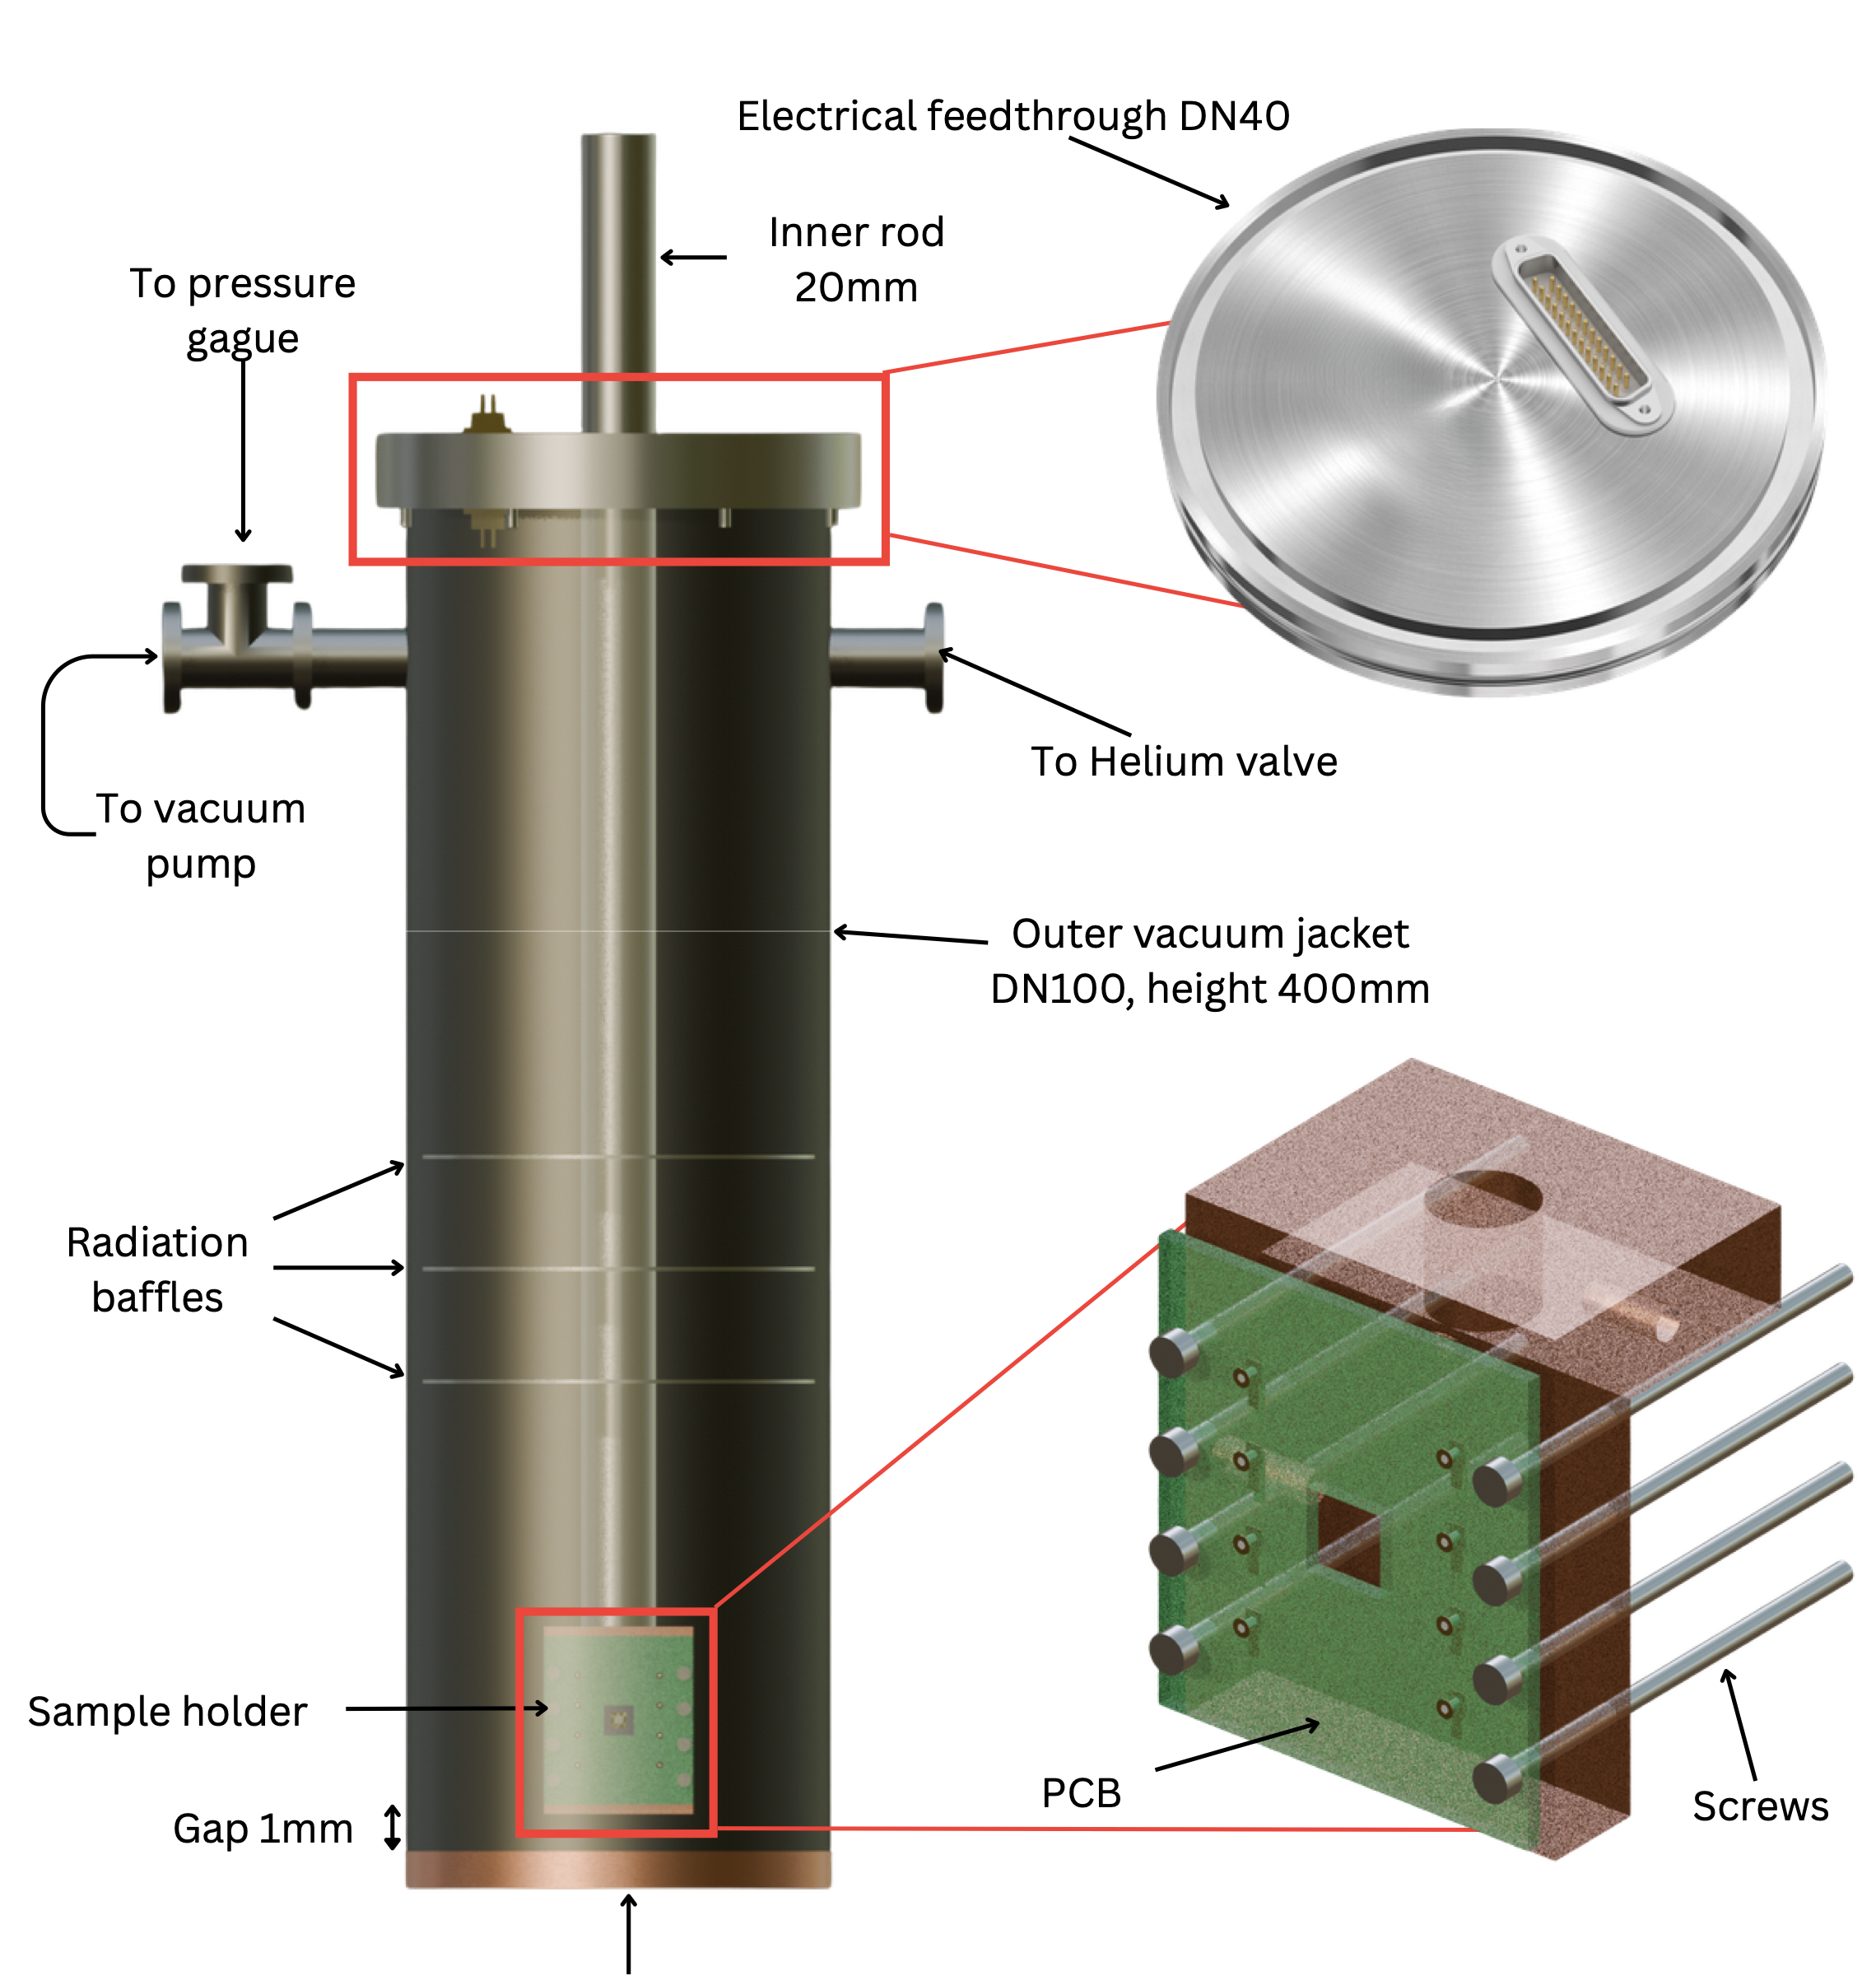
\includegraphics[width=0.92\linewidth]{cryostat_design_overview.png} \\
      \vspace{0.2cm}
      \small\textit{Full 3D cross-sectional CAD assembly of the cryostat.}
    \end{center}
    \vspace{0.4cm}
    \begin{itemize}
      \item \textbf{Modular Vacuum Enclosure:} SS304L body with standard KF-40 flanges, viton O-rings, and quick-release centering clamps.
      \item \textbf{Cryogenic Delivery Tube:} Continuous liquid nitrogen delivery tube entering the cold head with minimal parasitic conductive bridges.
    \end{itemize}
  }

  \block{4. Sample Stage \& 4-Probe Interface}{
    \begin{center}
      \begin{minipage}{0.48\linewidth}
        \centering
        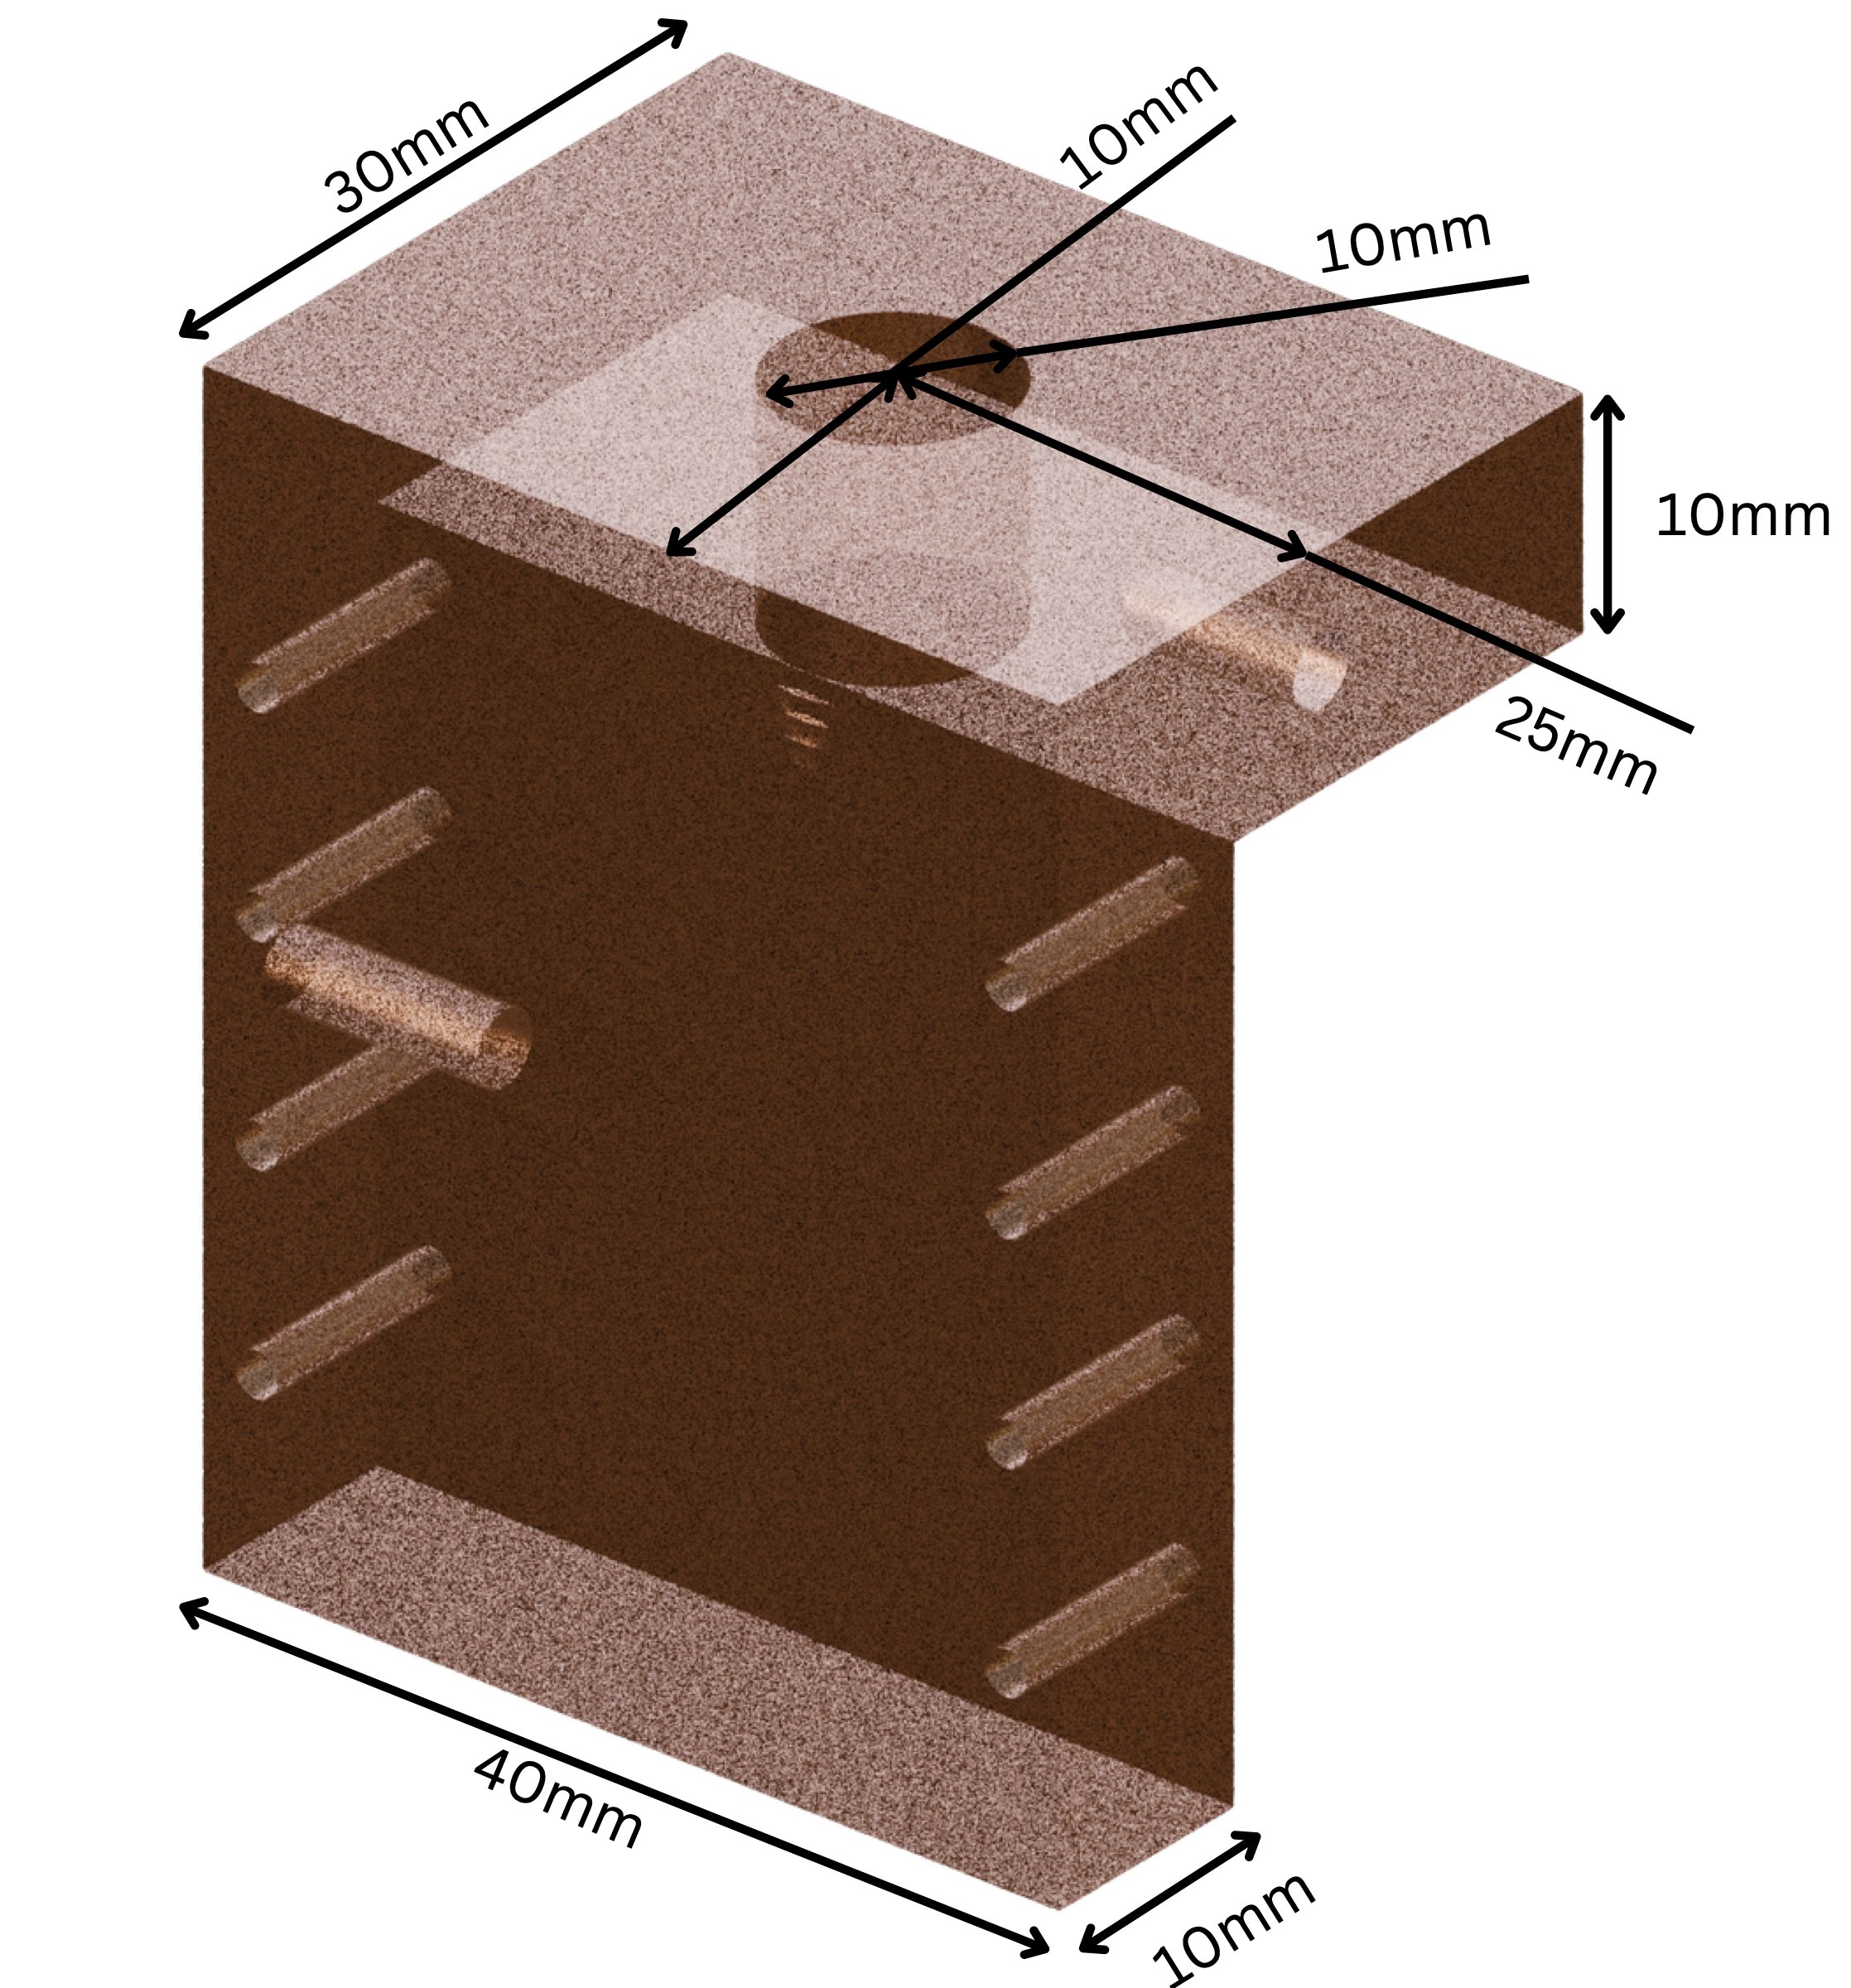
\includegraphics[width=\linewidth]{cryostat_holder_iso_3d.png} \\
        \small 3D OFHC sample stage
      \end{minipage}
      \hfill
      \begin{minipage}{0.48\linewidth}
        \centering
        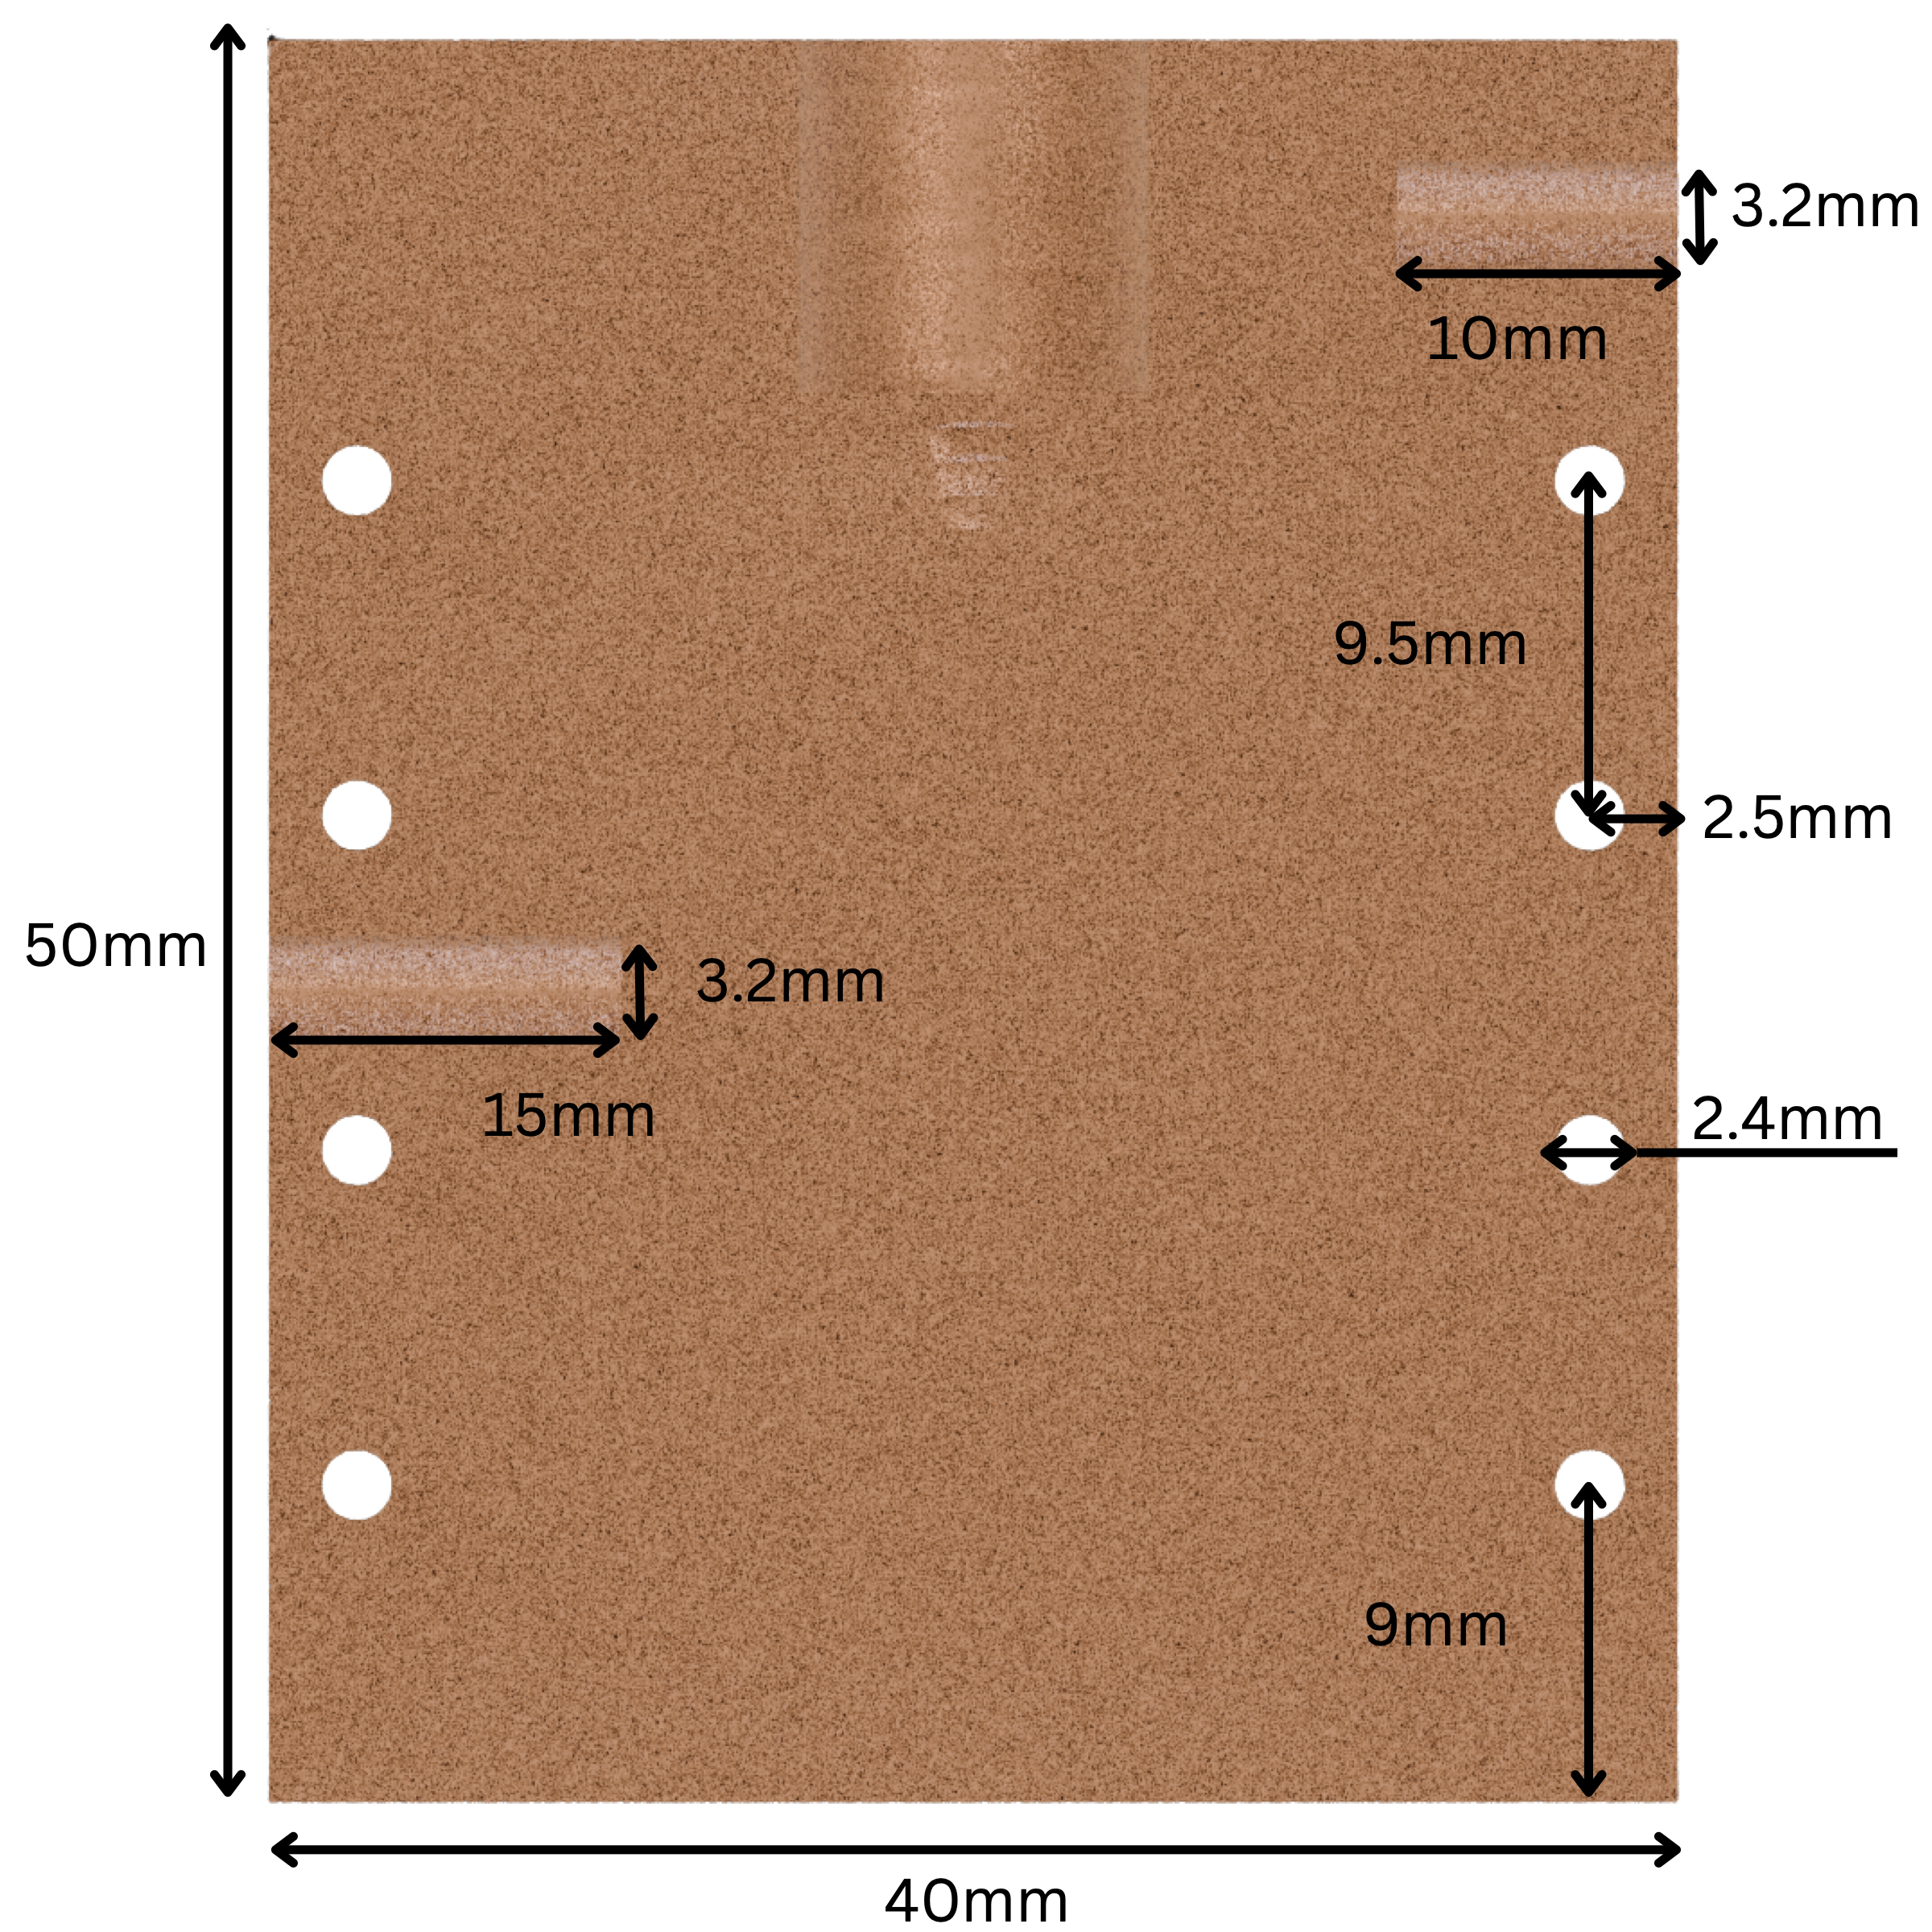
\includegraphics[width=\linewidth]{cryostat_holder_front_cad.png} \\
        \small FreeCAD engineering drawing
      \end{minipage}
    \end{center}
    \vspace{0.4cm}
    \begin{itemize}
      \item \textbf{L-Shaped Geometric Profile:} Optimizes conductive contact area with the cold finger while preserving optical and electrical top access.
      \item \textbf{Electrical Contact Interface:} Gold-plated phosphor-bronze spring probes mounted on a low-outgassing PCB base for 4-probe van der Pauw resistivity measurements.
    \end{itemize}
  }

  % ============================================================================
  % COLUMN 3: SIMULATION, EXPERIMENTAL & SPECS
  % ============================================================================
  \column{0.33}

  \block{5. Experimental Results \& Thermal PID}{
    \begin{center}
      \begin{minipage}{0.48\linewidth}
        \centering
        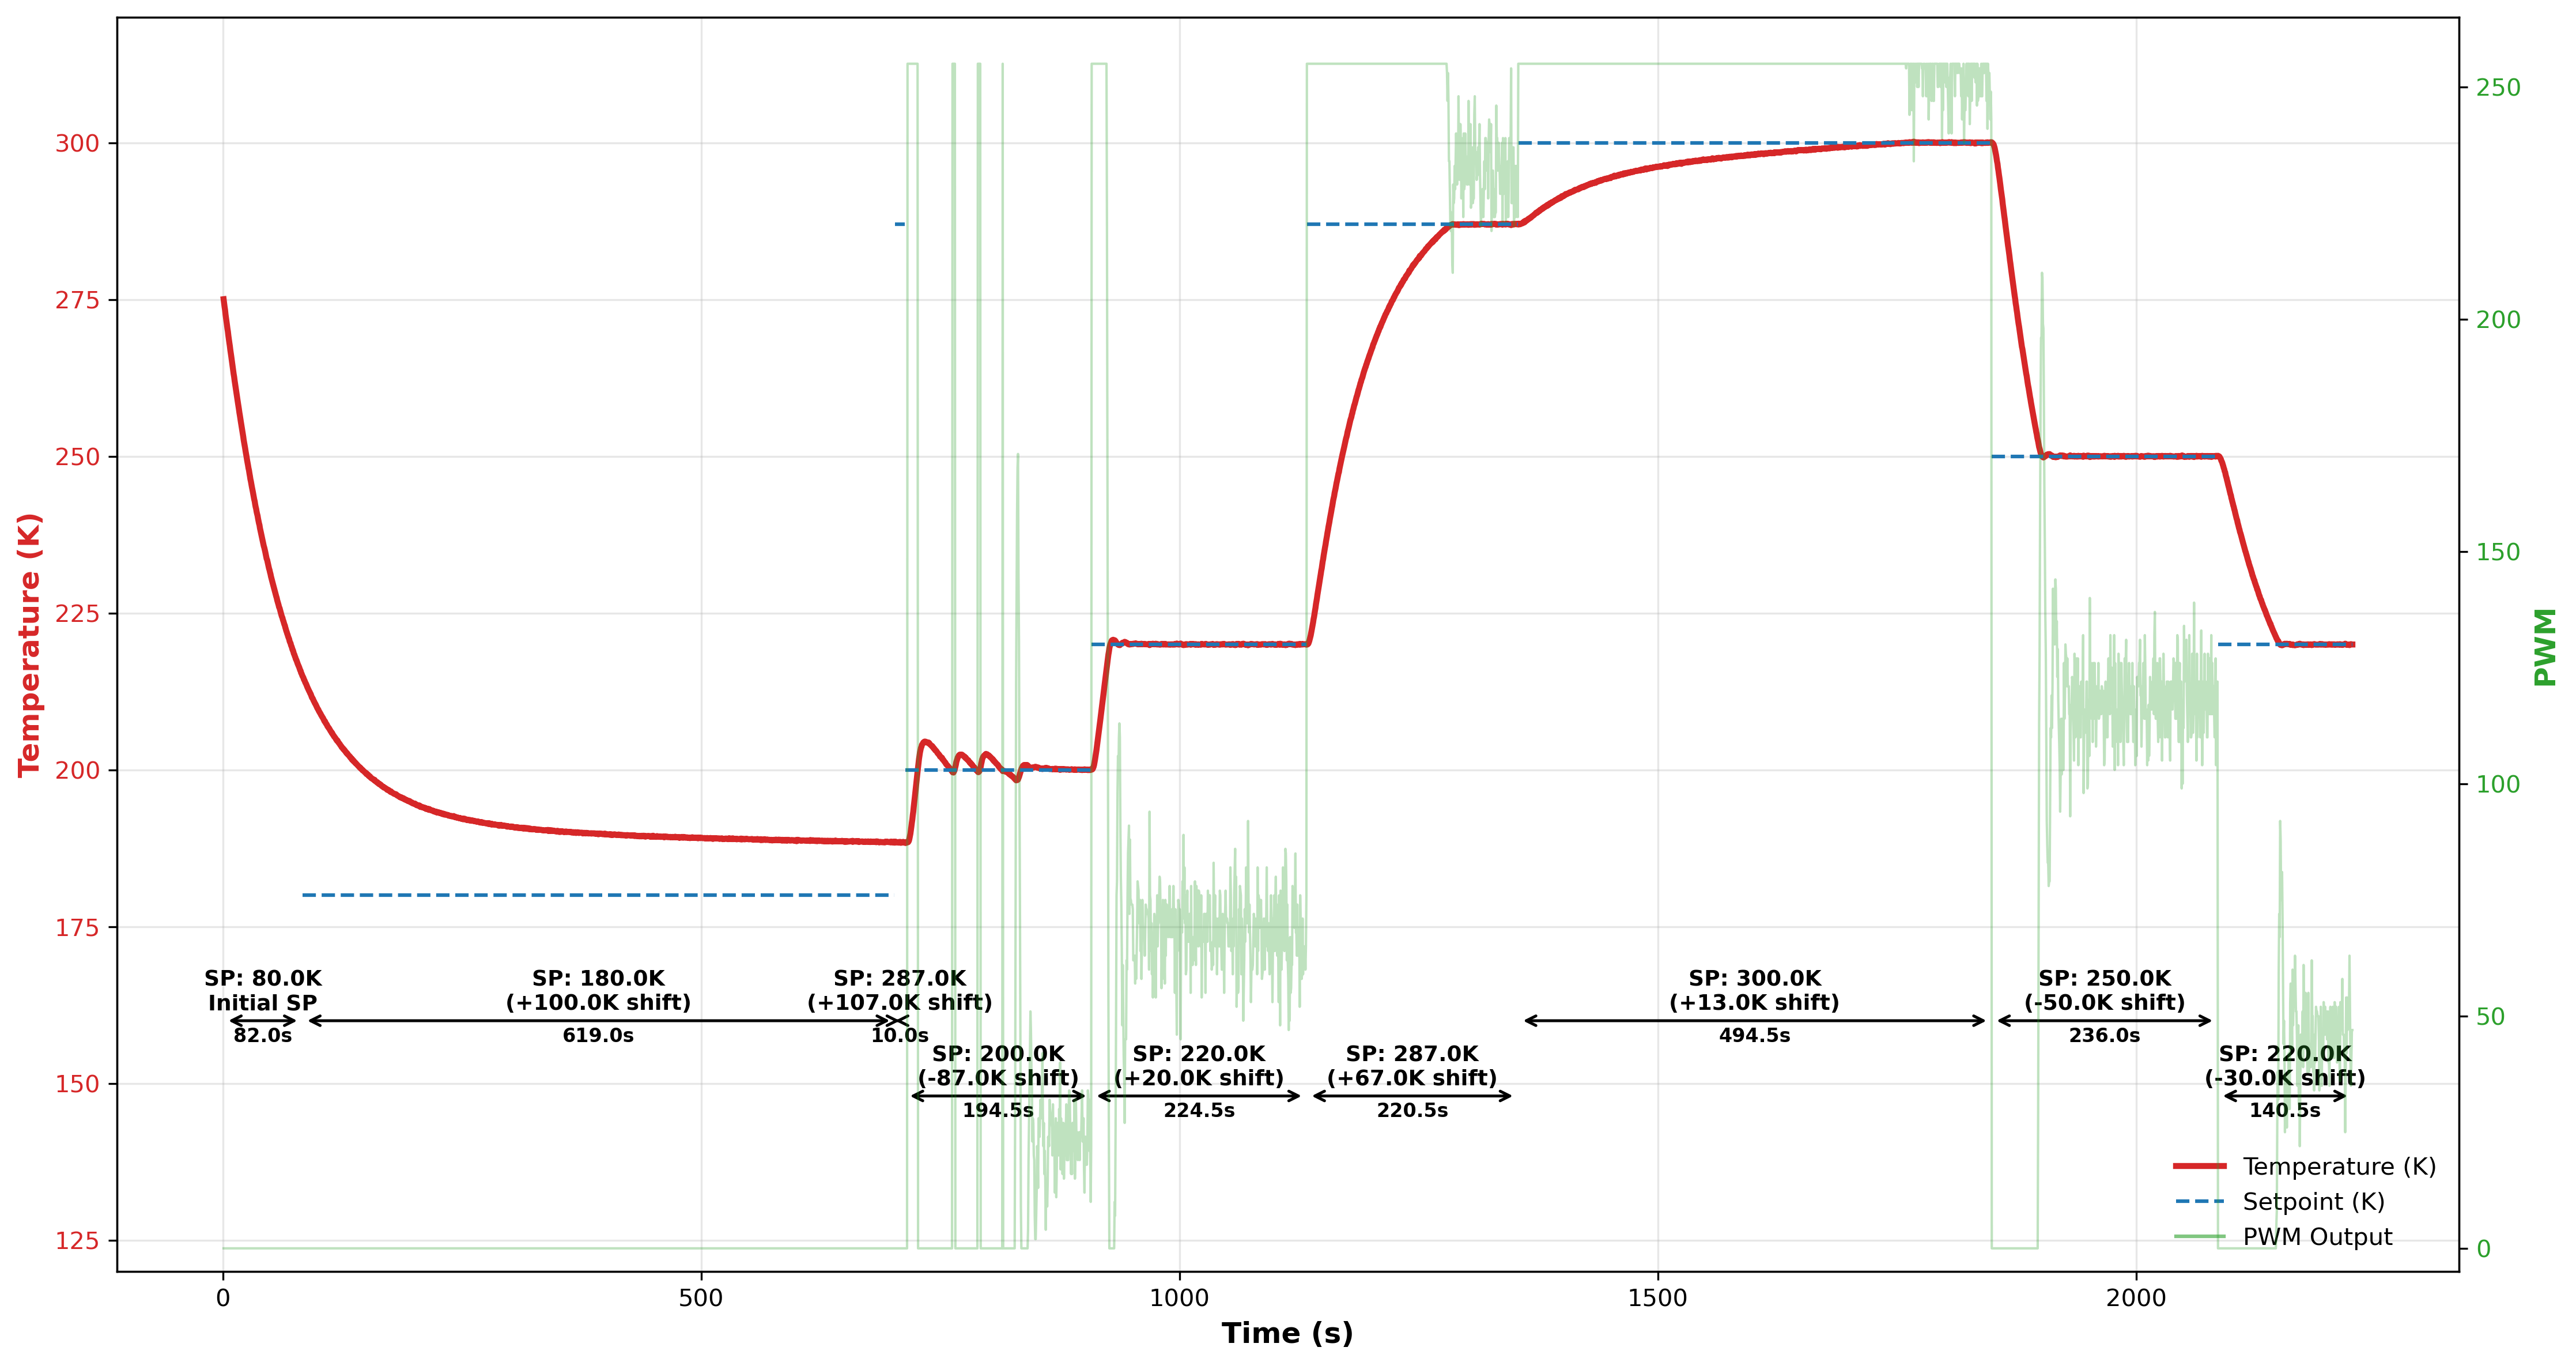
\includegraphics[width=\linewidth]{cryostat_cooling_curve.png} \\
        \small Continuous-flow cooldown
      \end{minipage}
      \hfill
      \begin{minipage}{0.48\linewidth}
        \centering
        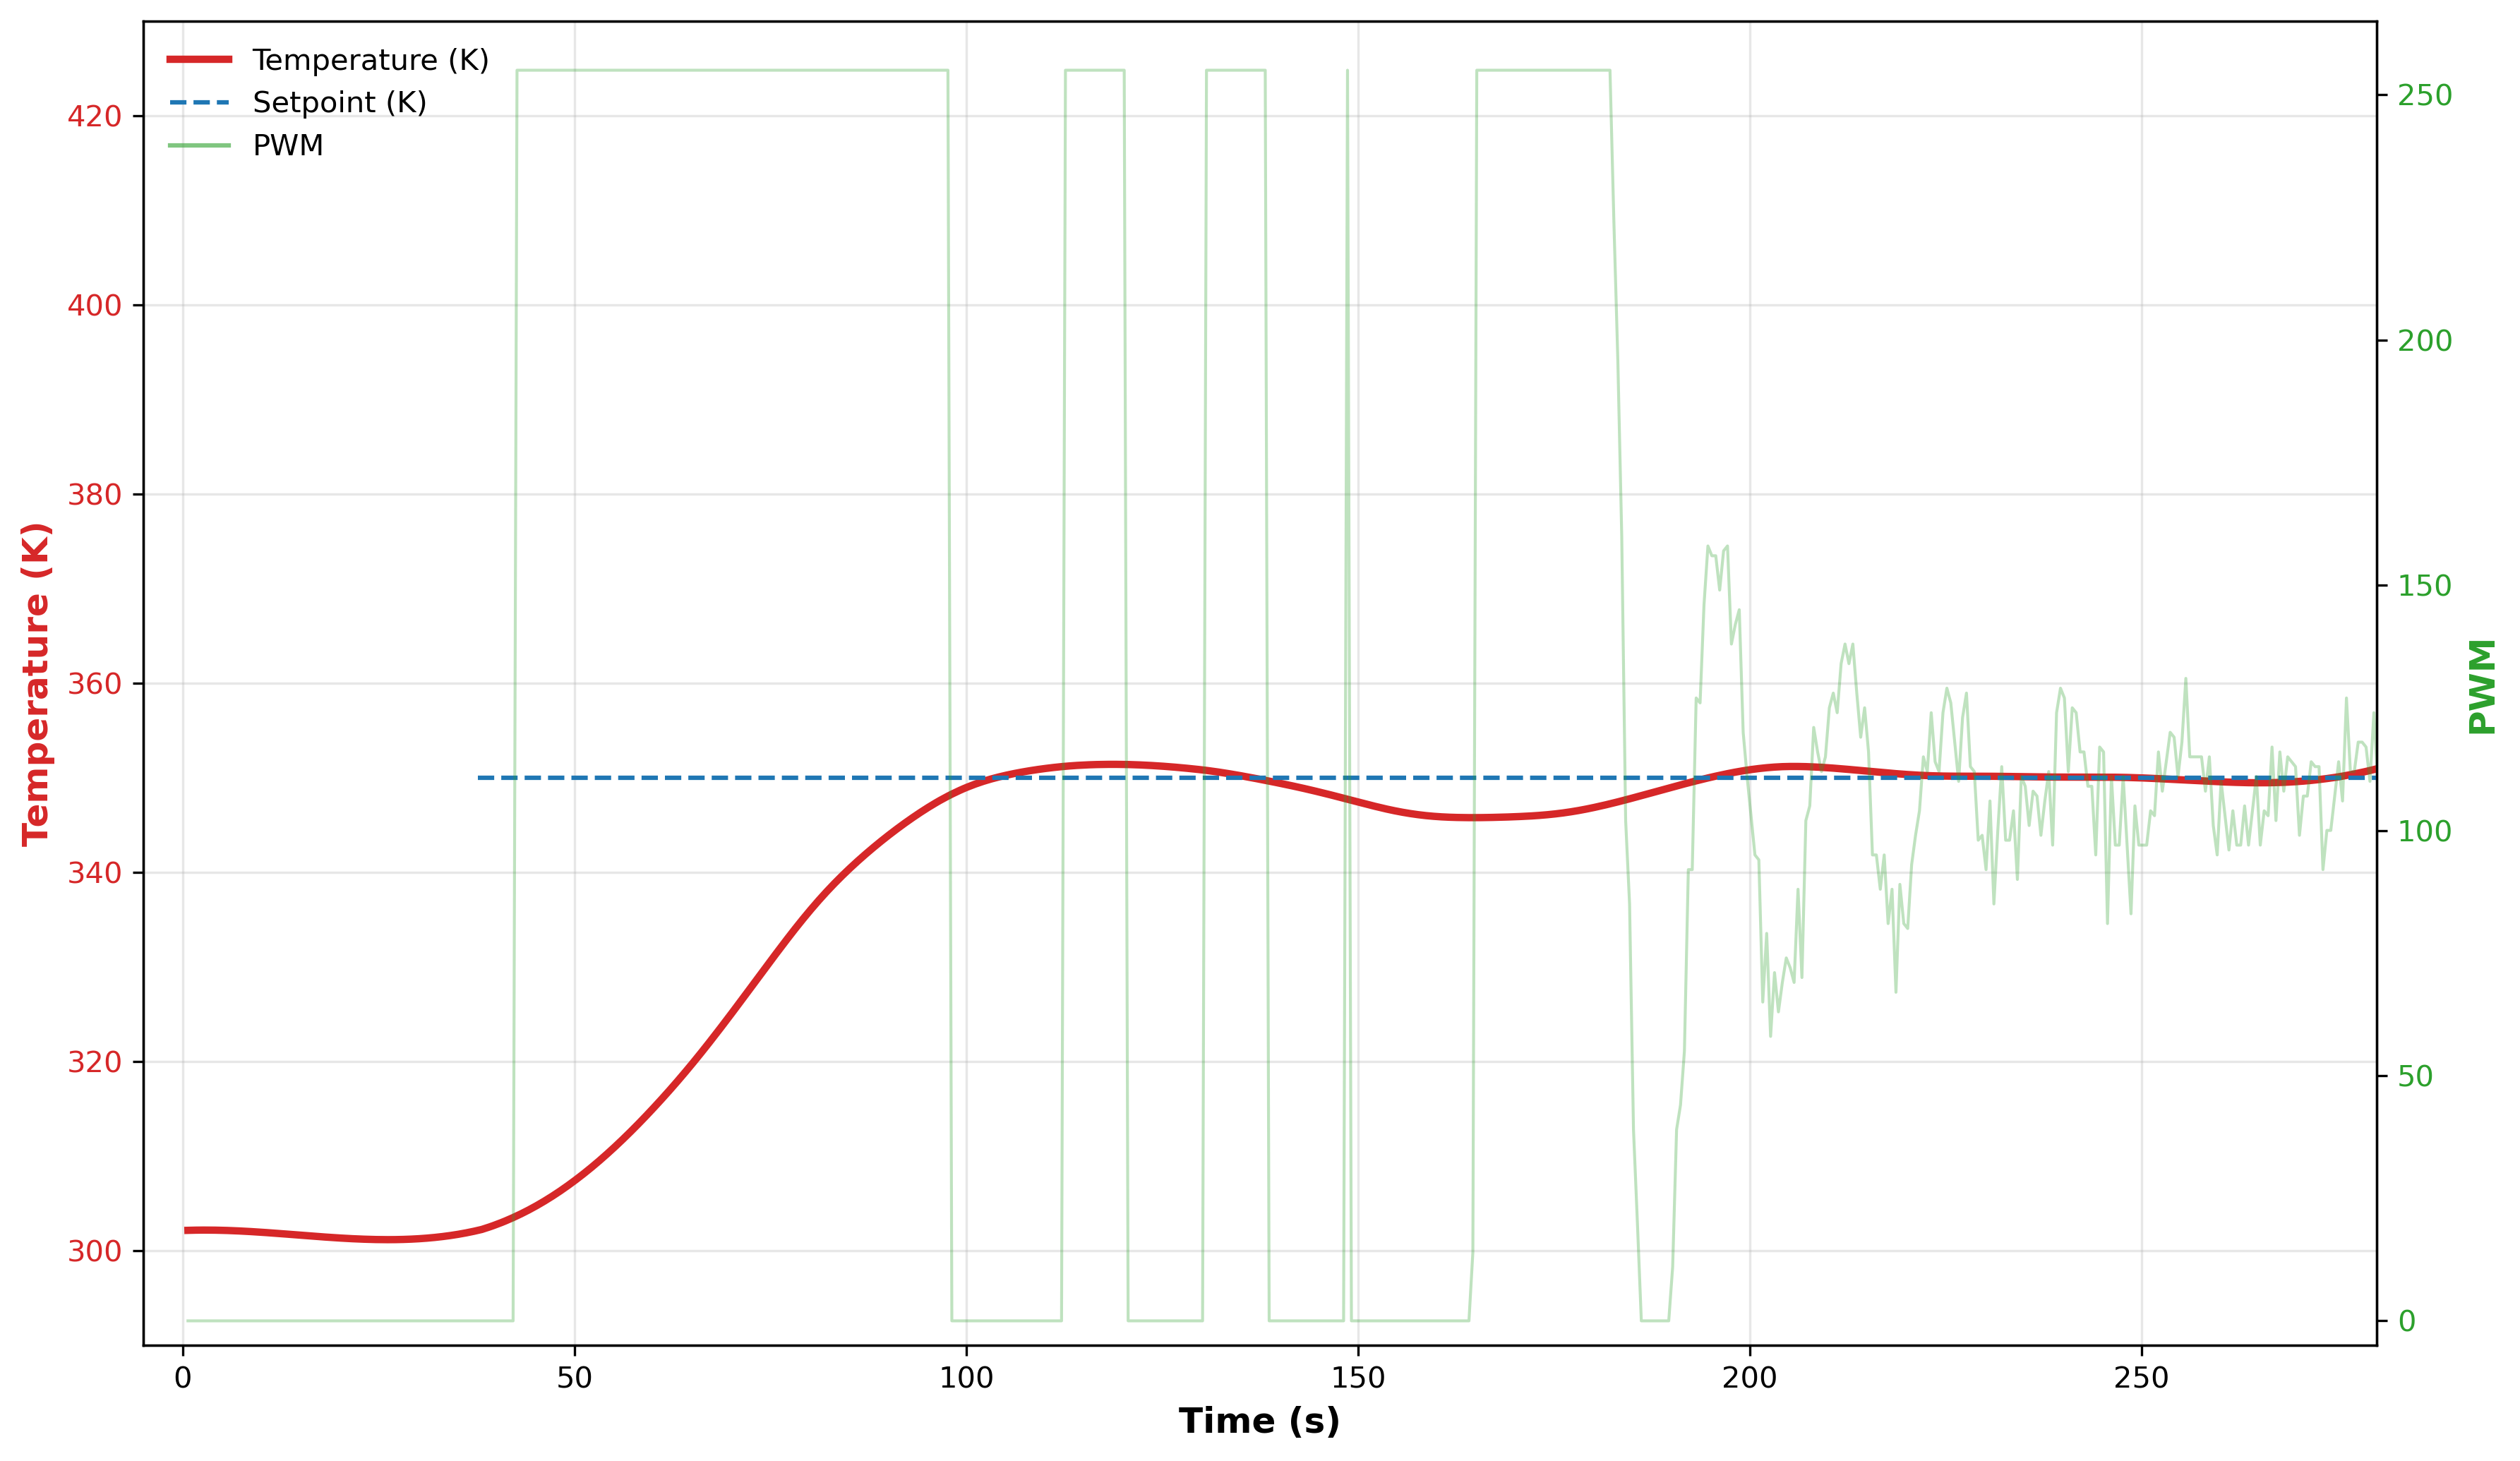
\includegraphics[width=\linewidth]{cryostat_vacuum_curve.png} \\
        \small Vacuum pump-down curve
      \end{minipage}
    \end{center}
    \vspace{0.3cm}
    \begin{center}
      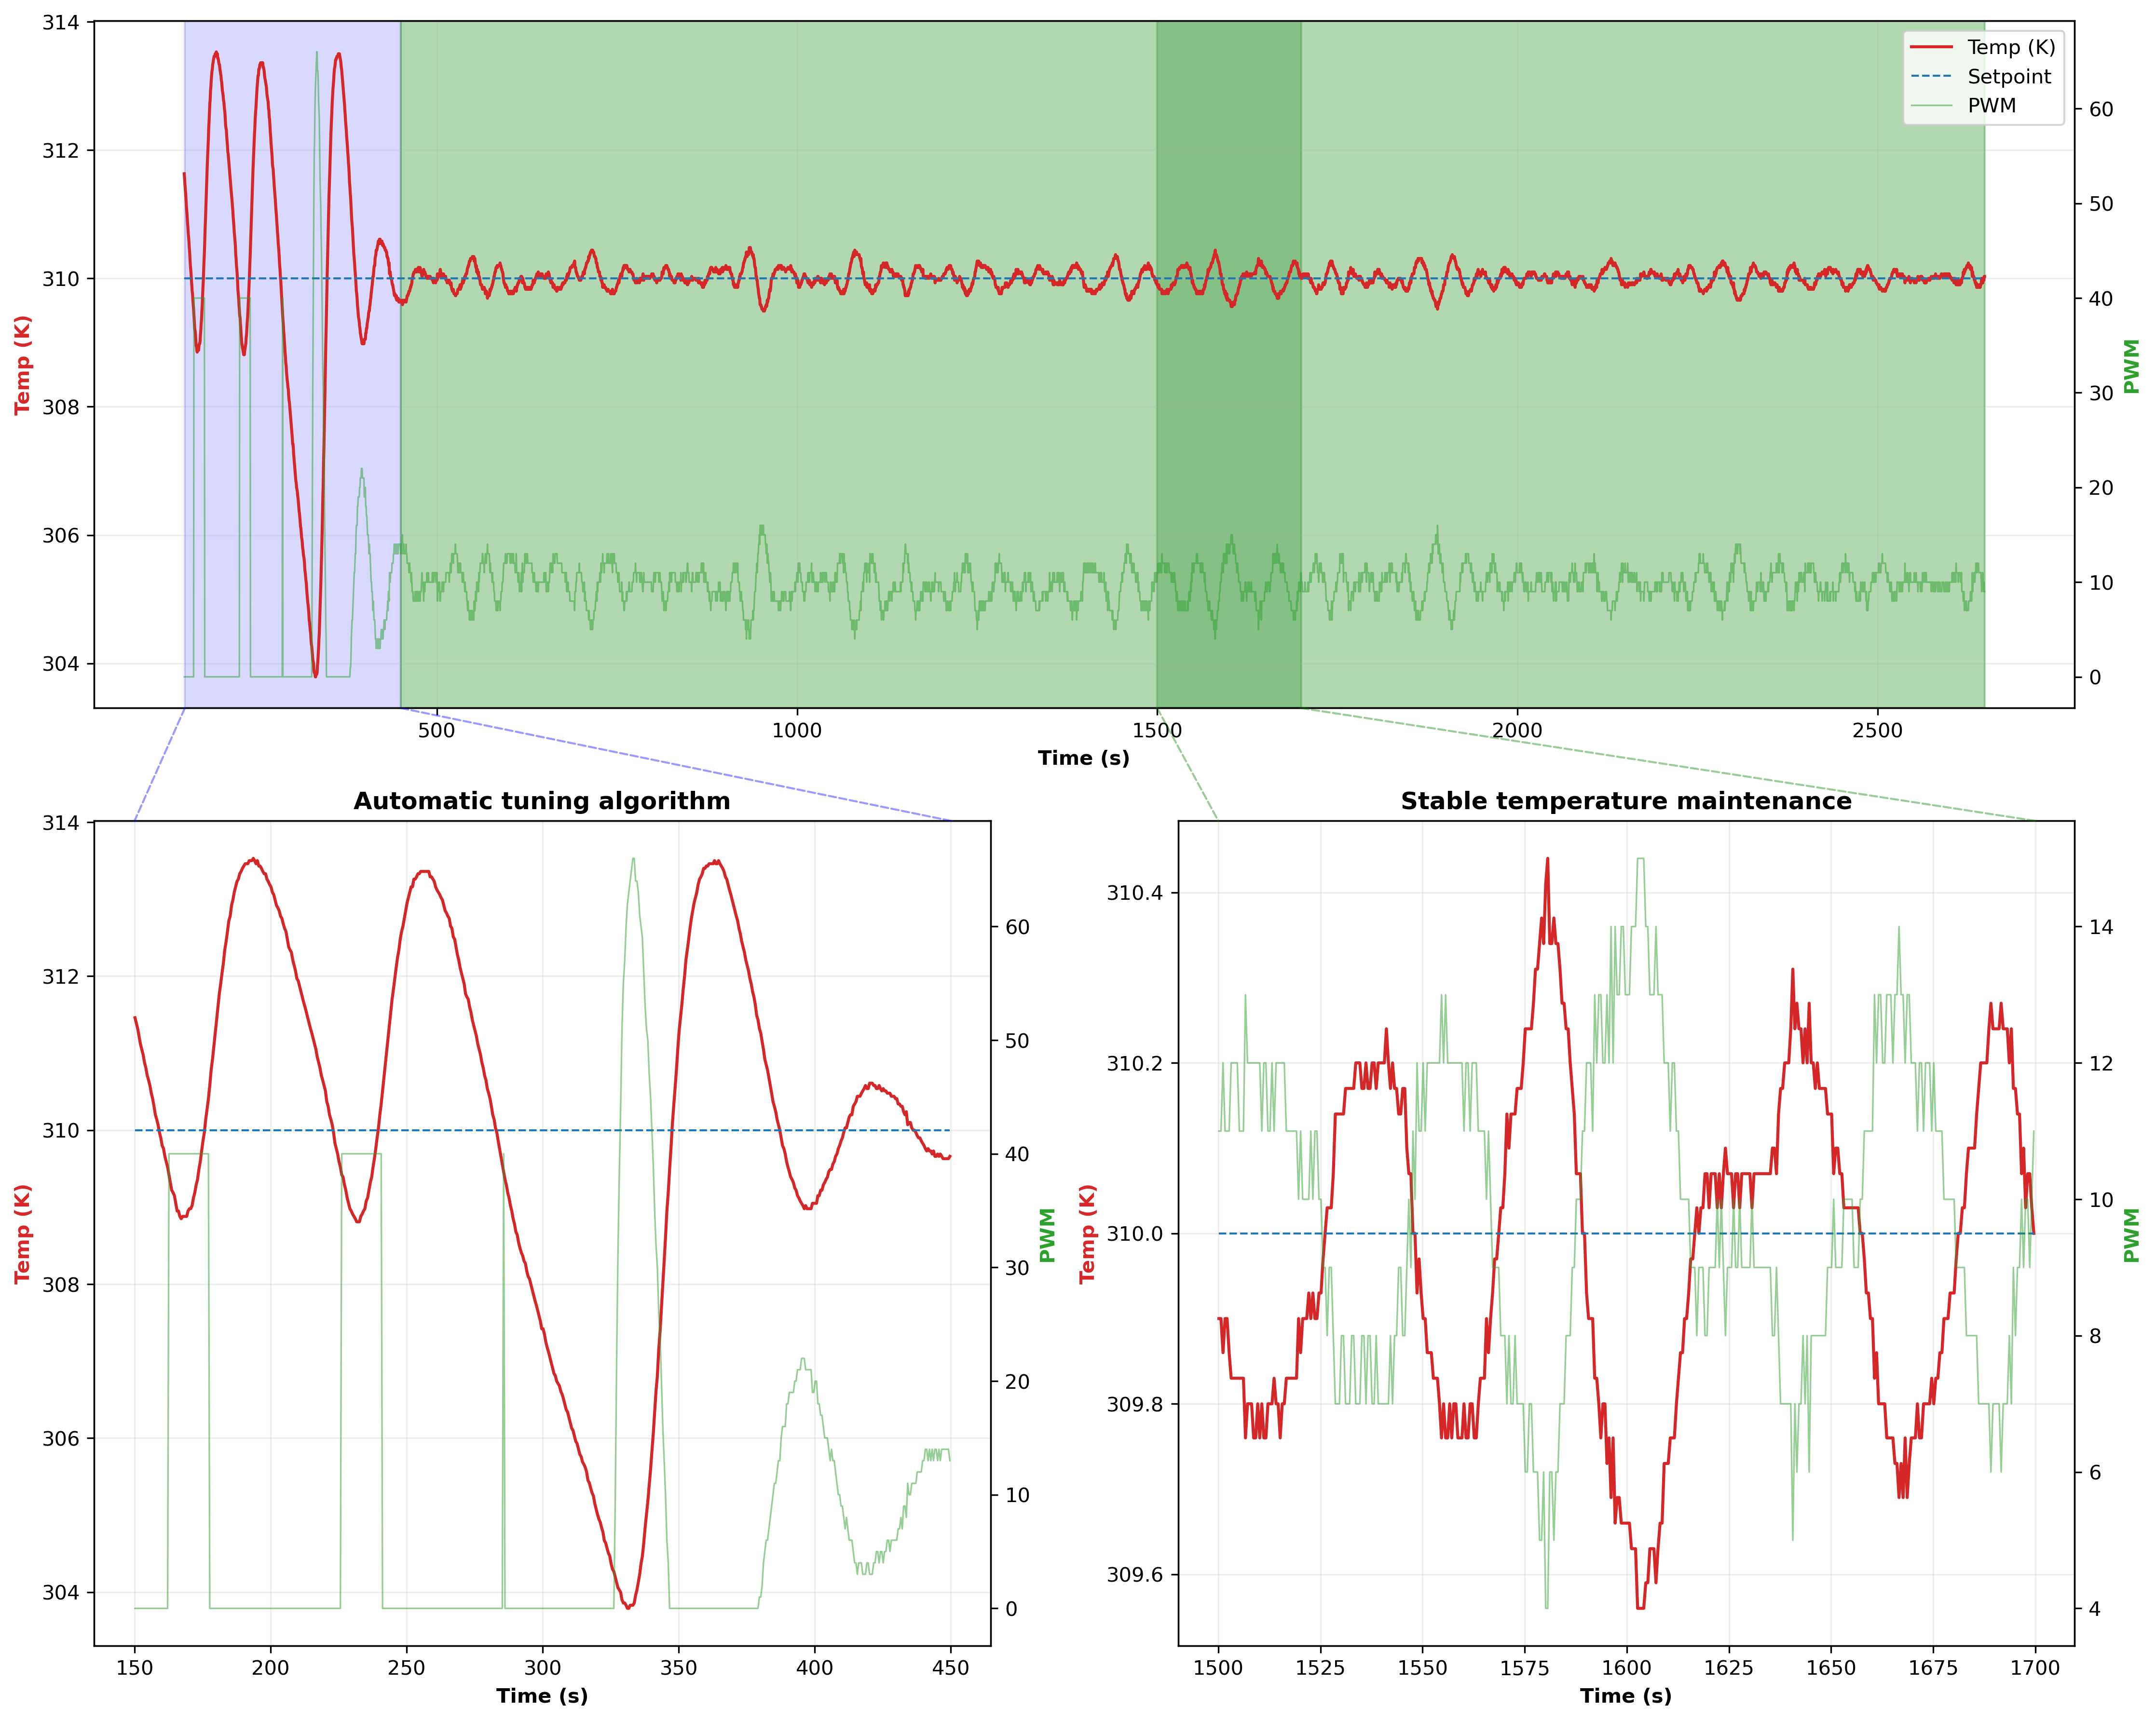
\includegraphics[width=0.92\linewidth]{cryostat_pid_stabilization.png} \\
      \small\textit{PID thermal regulation ($\pm 0.4\text{ K}$) across multi-step setpoints.}
    \end{center}
    \vspace{0.3cm}
    \begin{itemize}
      \item \textbf{Dynamic Thermal Tracking:} Åström-Hägglund relay auto-tuning with Tyreus-Luyben rules smoothly managed thermal inertia.
      \item \textbf{Thermal Stability:} Maintained setpoints with $\pm 0.4\text{ K}$ steady-state fluctuation from $160\text{ K}$ to $300\text{ K}$ without sustained oscillation.
    \end{itemize}
  }

  \block{6. System Specifications \& Conclusion}{
    \begin{center}
      \large
      \begin{tabular}{ll}
        \toprule
        \textbf{Parameter} & \textbf{Demonstrated Value} \\
        \midrule
        Temperature Range & $160\text{ K} - 300\text{ K}$ (Tested) / $77\text{ K}$ (Baseline LN2) \\
        Temperature Stability & $\pm 0.4\text{ K}$ steady-state fluctuation \\
        Ultimate Base Vacuum & $8.5 \times 10^{-5}\text{ mbar}$ (molecular flow regime) \\
        Sample Mount & OFHC copper stage with 4-probe spring pins \\
        Control Architecture & Arduino PID + Python GUI with live telemetry \\
        \bottomrule
      \end{tabular}
    \end{center}
    \vspace{0.4cm}
    \textbf{Conclusion:} Validated a robust, modular, open-source continuous-flow cryostat platform integrating high vacuum isolation, precision PID temperature regulation, and in-situ electrical resistivity characterization.
  }

\end{columns}

\end{document}
